\section{Simulation Study}
\label{sec:simulation}

\subsection{Design}

We study the method in a simulation setting with six scenarios that represent
different kinds of mismatch between the concurrent and external datasets.
SC1 is the fully exchangeable case.
SC2 and SC4 introduce covariate shift.
SC3 and SC5 introduce outcome drift.
SC6 combines both covariate shift and outcome drift.

For each scenario, we generate one concurrent dataset and one external dataset
using the model in Section~\ref{sec:problem}.
We consider $N_c \in \{50,100\}$ and fix $N_e=200$.
The target parameter is the current-study effect $\theta$.

\subsection{Methods compared}

The main text comparison includes four methods:
\begin{itemize}3
    \item \textbf{PSPower}, a propensity-score-stratified power prior;
    \item \textbf{IW}, an individualized weighting method;
    \item \textbf{Commensurate}, a commensurate-prior model;
    \item \textbf{NPE}, the proposed neural posterior estimation method.
\end{itemize}

OT- and KL-based extensions are not included in the main text.
We report those extensions in the appendix.

\subsection{Evaluation metrics}

We use two simulation settings.
In the non-null setting, we set $\theta=1$ and report bias, RMSE, coverage,
and power.
Bias and RMSE measure point estimation error.
Coverage checks whether the 95\% interval contains the true value.
Power is the fraction of 95\% intervals that exclude 0.

In the null setting, we set $\theta=0$ and report coverage and Type I error.
Type I error is the fraction of 95\% intervals that exclude 0 when the true
effect is zero.

\subsection{Main results for the non-null setting}

Table~\ref{tab:sim-main} shows the results for $\theta=1$.
Two patterns stand out.
First, in the easier settings, especially SC1 and SC2, the classical methods
already perform well, and NPE is somewhat more variable.
Second, once the outcome model differs across sources, the picture changes.
In SC3 and SC5, the classical borrowing methods have large bias and essentially
no coverage, while NPE remains much closer to the true target.
In SC6, where both covariate and outcome mismatch are present, NPE is
substantially more stable than PSPower and Commensurate, and is close to IW.

\begin{table*}[t]
\centering
\small
\caption{Non-null simulation results ($\theta = 1$).}
\label{tab:sim-main}
\begin{tabular}{llccccc}
\toprule
$N_c$ & Scenario & Method & Bias & RMSE & Coverage & Power \\
\midrule
\multirow{24}{*}{50}
& SC1 & PSPower      & 0.0183 & 0.1268 & 0.90 & 1.00 \\
& SC1 & IW           & 0.0365 & 0.1309 & 0.94 & 1.00 \\
& SC1 & Commensurate & 0.0183 & 0.1234 & 0.90 & 1.00 \\
& SC1 & NPE          & 0.2201 & 0.3049 & 0.94 & 1.00 \\
\cmidrule(lr){2-7}
& SC2 & PSPower      & -0.0126 & 0.1485 & 0.94 & 1.00 \\
& SC2 & IW           & -0.0223 & 0.1505 & 0.98 & 1.00 \\
& SC2 & Commensurate & -0.0160 & 0.1464 & 0.94 & 1.00 \\
& SC2 & NPE          & 0.2202 & 0.3219 & 0.92 & 1.00 \\
\cmidrule(lr){2-7}
& SC3 & PSPower      & 1.1655 & 1.1693 & 0.00 & 1.00 \\
& SC3 & IW           & 0.9306 & 0.9369 & 0.00 & 1.00 \\
& SC3 & Commensurate & 1.1016 & 1.1091 & 0.00 & 1.00 \\
& SC3 & NPE          & 0.1889 & 0.2859 & 0.98 & 1.00 \\
\cmidrule(lr){2-7}
& SC4 & PSPower      & 0.0432 & 0.1579 & 0.94 & 1.00 \\
& SC4 & IW           & 0.0394 & 0.1697 & 0.98 & 1.00 \\
& SC4 & Commensurate & 0.0347 & 0.1630 & 0.94 & 1.00 \\
& SC4 & NPE          & 0.2661 & 0.3570 & 0.92 & 1.00 \\
\cmidrule(lr){2-7}
& SC5 & PSPower      & 1.1936 & 1.1993 & 0.00 & 1.00 \\
& SC5 & IW           & 0.9810 & 0.9915 & 0.00 & 1.00 \\
& SC5 & Commensurate & 1.1399 & 1.1488 & 0.00 & 1.00 \\
& SC5 & NPE          & 0.2298 & 0.3115 & 0.94 & 1.00 \\
\cmidrule(lr){2-7}
& SC6 & PSPower      & 0.5617 & 0.5943 & 0.08 & 1.00 \\
& SC6 & IW           & 0.2521 & 0.3167 & 0.68 & 1.00 \\
& SC6 & Commensurate & 0.4765 & 0.5107 & 0.16 & 1.00 \\
& SC6 & NPE          & 0.1311 & 0.2523 & 0.98 & 1.00 \\
\midrule
\multirow{24}{*}{100}
& SC1 & PSPower      & 0.0178 & 0.1063 & 0.94 & 1.00 \\
& SC1 & IW           & 0.0238 & 0.1205 & 0.98 & 1.00 \\
& SC1 & Commensurate & 0.0183 & 0.1058 & 0.92 & 1.00 \\
& SC1 & NPE          & 0.1413 & 0.2270 & 0.98 & 1.00 \\
\cmidrule(lr){2-7}
& SC2 & PSPower      & 0.0032 & 0.1261 & 0.94 & 1.00 \\
& SC2 & IW           & 0.0044 & 0.1422 & 0.94 & 1.00 \\
& SC2 & Commensurate & 0.0081 & 0.1195 & 0.94 & 1.00 \\
& SC2 & NPE          & 0.1610 & 0.2532 & 0.98 & 1.00 \\
\cmidrule(lr){2-7}
& SC3 & PSPower      & 0.9587 & 0.9651 & 0.00 & 1.00 \\
& SC3 & IW           & 0.6597 & 0.6701 & 0.00 & 1.00 \\
& SC3 & Commensurate & 0.8586 & 0.8714 & 0.00 & 1.00 \\
& SC3 & NPE          & 0.1518 & 0.2089 & 1.00 & 1.00 \\
\cmidrule(lr){2-7}
& SC4 & PSPower      & 0.0125 & 0.1576 & 0.86 & 1.00 \\
& SC4 & IW           & 0.0013 & 0.1552 & 0.90 & 1.00 \\
& SC4 & Commensurate & 0.0047 & 0.1497 & 0.90 & 1.00 \\
& SC4 & NPE          & 0.1312 & 0.2352 & 1.00 & 1.00 \\
\cmidrule(lr){2-7}
& SC5 & PSPower      & 0.9547 & 0.9597 & 0.00 & 1.00 \\
& SC5 & IW           & 0.6557 & 0.6681 & 0.00 & 1.00 \\
& SC5 & Commensurate & 0.8564 & 0.8710 & 0.00 & 1.00 \\
& SC5 & NPE          & 0.1299 & 0.1998 & 1.00 & 1.00 \\
\cmidrule(lr){2-7}
& SC6 & PSPower      & 0.3222 & 0.3595 & 0.32 & 1.00 \\
& SC6 & IW           & 0.0733 & 0.1672 & 0.92 & 1.00 \\
& SC6 & Commensurate & 0.2075 & 0.2633 & 0.54 & 1.00 \\
& SC6 & NPE          & 0.0668 & 0.1835 & 0.98 & 1.00 \\
\bottomrule
\end{tabular}
\end{table*}

Figures~\ref{fig:sim-bias}--\ref{fig:sim-power} show the same results.
To keep the main text simple, we show bias, RMSE, coverage, and power in the
figures.

\begin{figure}[!htbp]
    \centering
    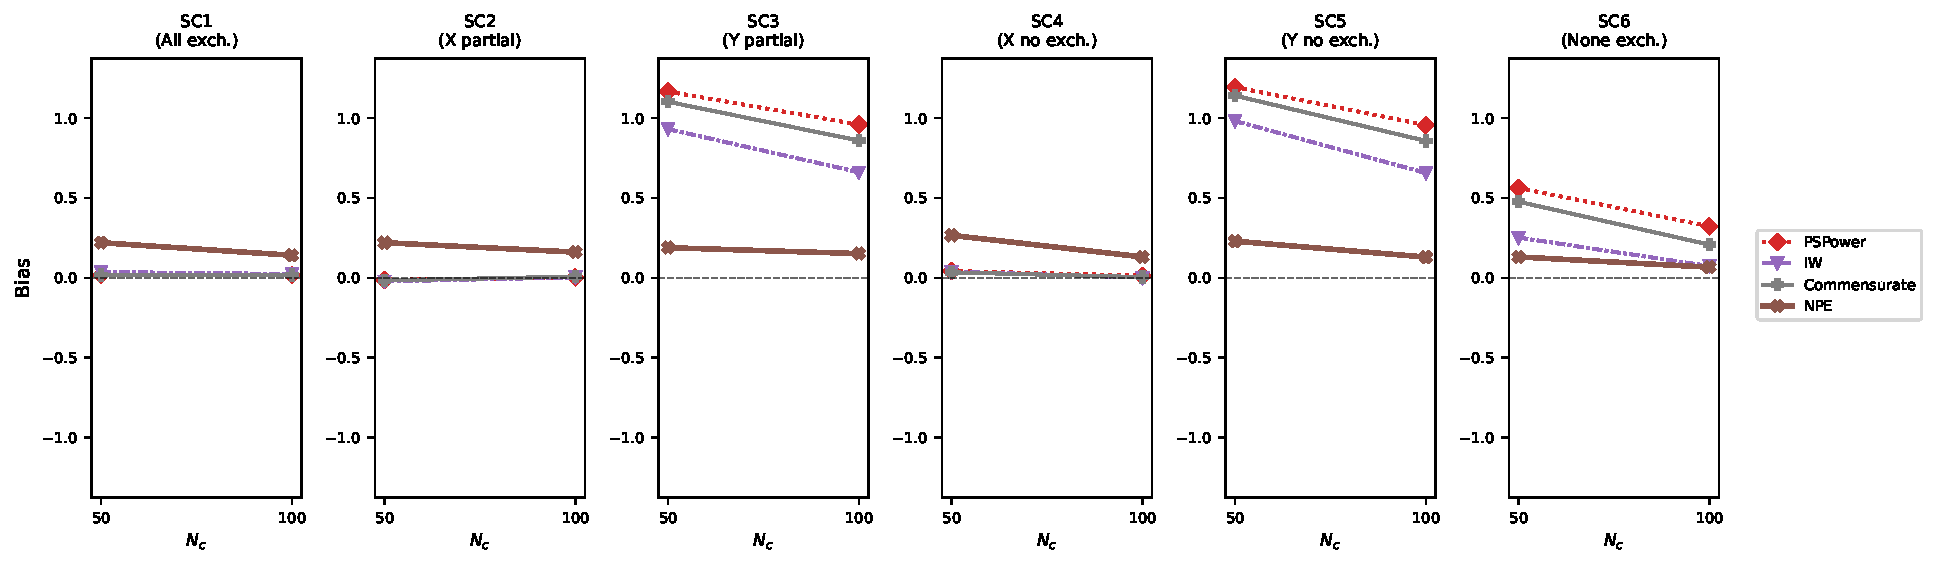
\includegraphics[width=.74\textwidth]{fig_bias.pdf}
    \caption{Bias across the six simulation scenarios for the non-null run.}
    \label{fig:sim-bias}
\end{figure}

\begin{figure}[!htbp]
    \centering
    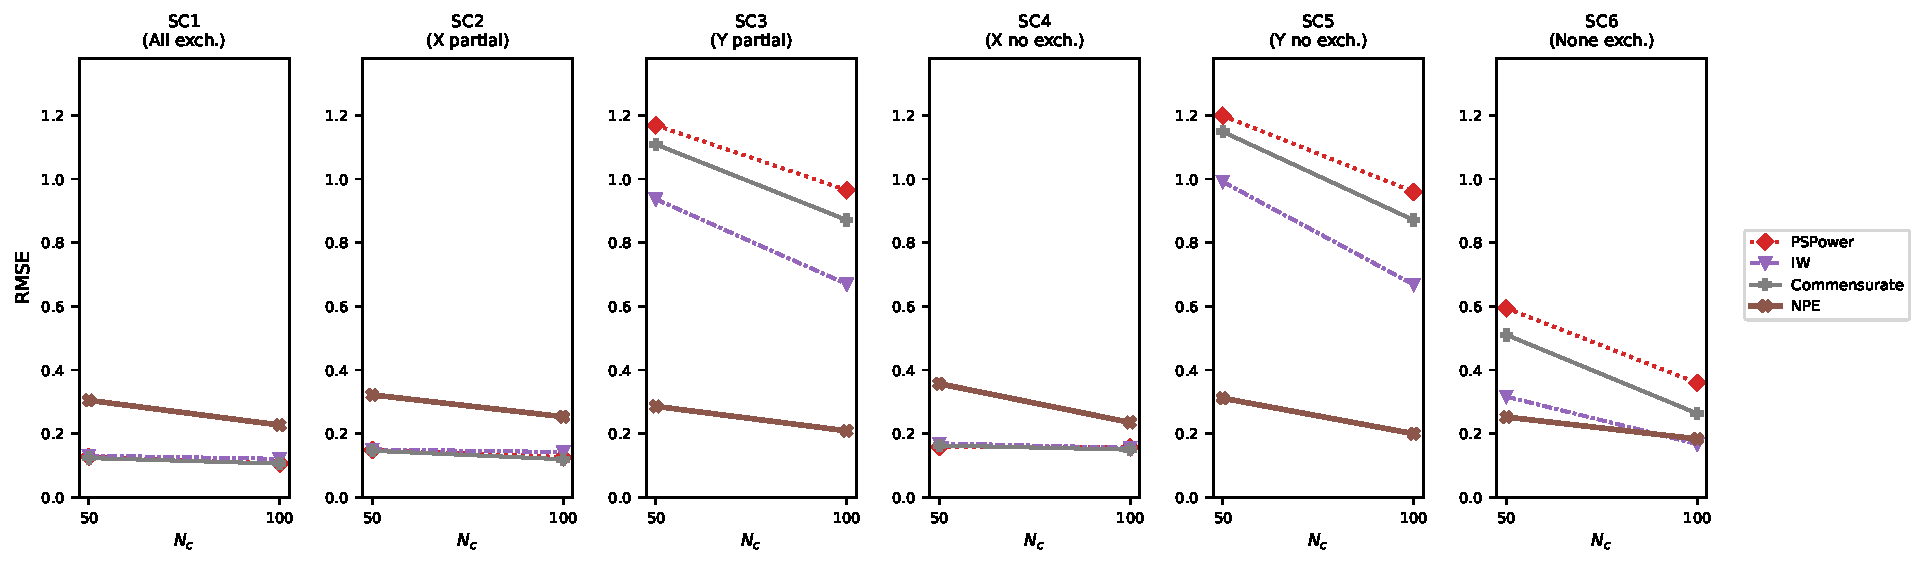
\includegraphics[width=.74\textwidth]{fig_rmse.pdf}
    \caption{RMSE across the six simulation scenarios for the non-null run.}
    \label{fig:sim-rmse}
\end{figure}

\begin{figure}[!htbp]
    \centering
    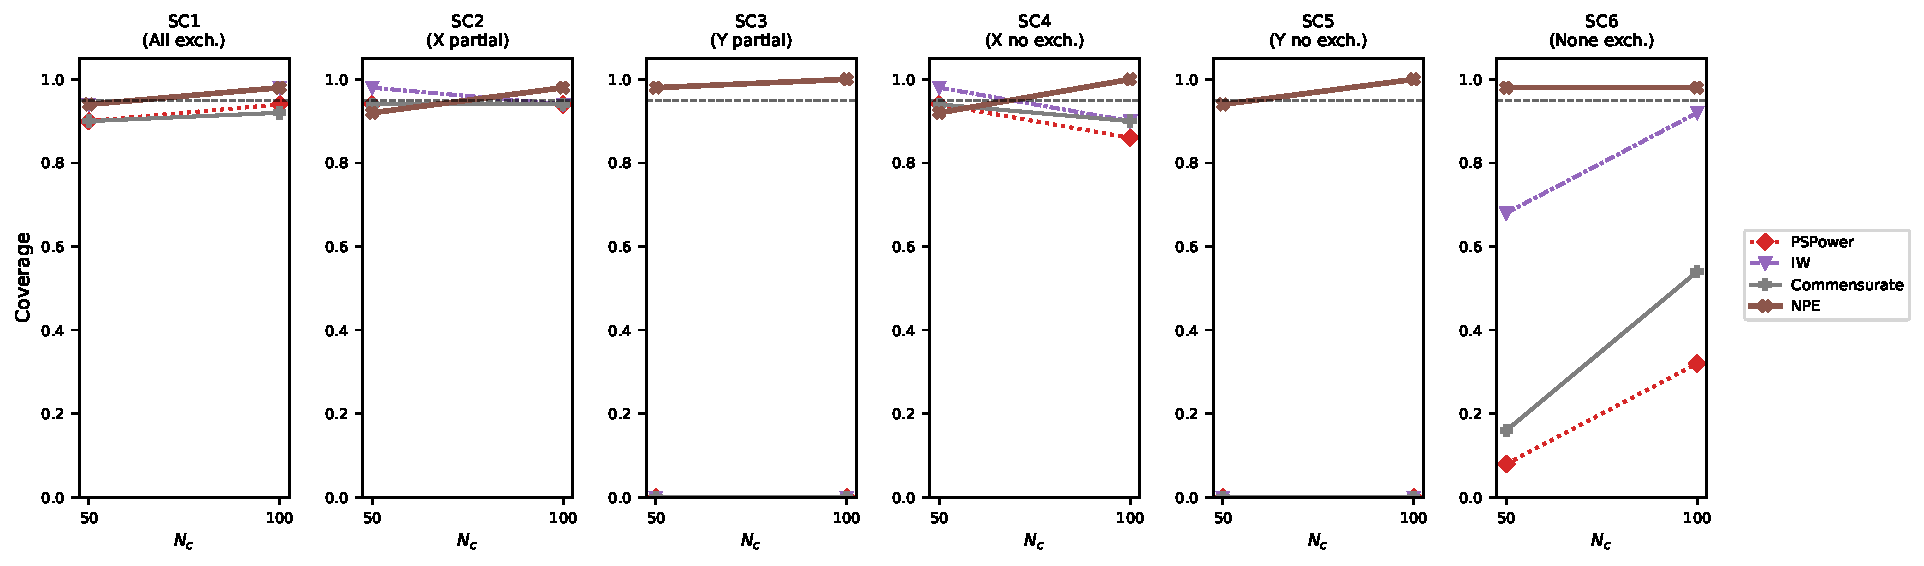
\includegraphics[width=.74\textwidth]{fig_coverage.pdf}
    \caption{Coverage across the six simulation scenarios for the non-null run.}
    \label{fig:sim-coverage}
\end{figure}

\begin{figure}[!htbp]
    \centering
    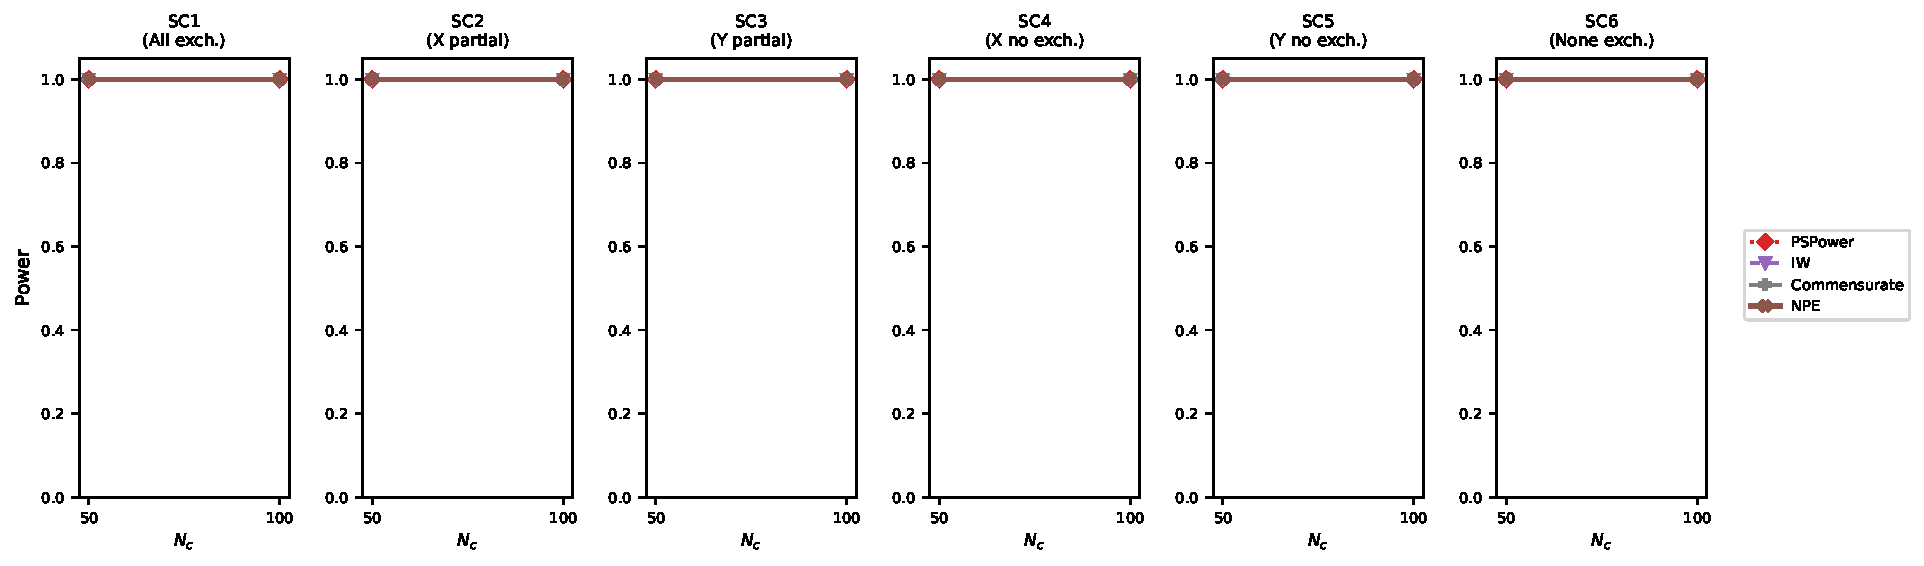
\includegraphics[width=.74\textwidth]{fig_power.pdf}
    \caption{Power across the six simulation scenarios for the non-null run.}
    \label{fig:sim-power}
\end{figure}

\subsection{Null results}

Table~\ref{tab:sim-null} summarizes the null run with $\theta=0$.
Here the main quantity of interest is Type I error.
In SC1 and SC2, the classical methods still have cleaner operating
characteristics, although NPE remains in a reasonable range.
The harder settings tell a different story.
In SC3, SC5, and SC6, the classical borrowing methods have very poor coverage
and severely inflated Type I error, while NPE stays much closer to nominal
behavior.

\begin{table*}[t]
\centering
\small
\caption{Null simulation results ($\theta = 0$).}
\label{tab:sim-null}
\begin{tabular}{llcccc}
\toprule
$N_c$ & Scenario & Method & Bias & RMSE & Coverage & Type I Error \\
\midrule
\multirow{24}{*}{50}
& SC1 & PSPower      & 0.0187 & 0.1269 & 0.90 & 0.10 \\
& SC1 & IW           & 0.0373 & 0.1311 & 0.94 & 0.06 \\
& SC1 & Commensurate & 0.0187 & 0.1235 & 0.90 & 0.10 \\
& SC1 & NPE          & 0.3172 & 0.3811 & 0.90 & 0.10 \\
\cmidrule(lr){2-7}
& SC2 & PSPower      & -0.0117 & 0.1485 & 0.94 & 0.06 \\
& SC2 & IW           & -0.0212 & 0.1503 & 0.98 & 0.02 \\
& SC2 & Commensurate & -0.0152 & 0.1463 & 0.94 & 0.06 \\
& SC2 & NPE          & 0.2954 & 0.3703 & 0.90 & 0.10 \\
\cmidrule(lr){2-7}
& SC3 & PSPower      & 1.1659 & 1.1698 & 0.00 & 1.00 \\
& SC3 & IW           & 0.9314 & 0.9377 & 0.00 & 1.00 \\
& SC3 & Commensurate & 1.1022 & 1.1096 & 0.00 & 1.00 \\
& SC3 & NPE          & 0.3333 & 0.4062 & 0.92 & 0.08 \\
\cmidrule(lr){2-7}
& SC4 & PSPower      & 0.0441 & 0.1582 & 0.96 & 0.04 \\
& SC4 & IW           & 0.0406 & 0.1700 & 0.98 & 0.02 \\
& SC4 & Commensurate & 0.0355 & 0.1632 & 0.94 & 0.06 \\
& SC4 & NPE          & 0.3495 & 0.4082 & 0.86 & 0.14 \\
\cmidrule(lr){2-7}
& SC5 & PSPower      & 1.1941 & 1.1997 & 0.00 & 1.00 \\
& SC5 & IW           & 0.9817 & 0.9923 & 0.00 & 1.00 \\
& SC5 & Commensurate & 1.1404 & 1.1493 & 0.00 & 1.00 \\
& SC5 & NPE          & 0.4052 & 0.4649 & 0.84 & 0.16 \\
\cmidrule(lr){2-7}
& SC6 & PSPower      & 0.5626 & 0.5952 & 0.08 & 0.92 \\
& SC6 & IW           & 0.2533 & 0.3176 & 0.68 & 0.32 \\
& SC6 & Commensurate & 0.4774 & 0.5114 & 0.18 & 0.82 \\
& SC6 & NPE          & 0.2874 & 0.3508 & 0.92 & 0.08 \\
\midrule
\multirow{24}{*}{100}
& SC1 & PSPower      & 0.0182 & 0.1063 & 0.94 & 0.06 \\
& SC1 & IW           & 0.0245 & 0.1206 & 0.98 & 0.02 \\
& SC1 & Commensurate & 0.0187 & 0.1059 & 0.92 & 0.08 \\
& SC1 & NPE          & 0.2542 & 0.3022 & 0.92 & 0.08 \\
\cmidrule(lr){2-7}
& SC2 & PSPower      & 0.0039 & 0.1262 & 0.94 & 0.06 \\
& SC2 & IW           & 0.0052 & 0.1422 & 0.94 & 0.06 \\
& SC2 & Commensurate & 0.0087 & 0.1195 & 0.94 & 0.06 \\
& SC2 & NPE          & 0.3132 & 0.3690 & 0.92 & 0.08 \\
\cmidrule(lr){2-7}
& SC3 & PSPower      & 0.9591 & 0.9655 & 0.00 & 1.00 \\
& SC3 & IW           & 0.6603 & 0.6707 & 0.00 & 1.00 \\
& SC3 & Commensurate & 0.8593 & 0.8721 & 0.00 & 1.00 \\
& SC3 & NPE          & 0.3574 & 0.3776 & 0.98 & 0.02 \\
\cmidrule(lr){2-7}
& SC4 & PSPower      & 0.0132 & 0.1576 & 0.86 & 0.14 \\
& SC4 & IW           & 0.0021 & 0.1551 & 0.92 & 0.08 \\
& SC4 & Commensurate & 0.0053 & 0.1497 & 0.90 & 0.10 \\
& SC4 & NPE          & 0.2651 & 0.3219 & 0.98 & 0.02 \\
\cmidrule(lr){2-7}
& SC5 & PSPower      & 0.9551 & 0.9601 & 0.00 & 1.00 \\
& SC5 & IW           & 0.6563 & 0.6687 & 0.00 & 1.00 \\
& SC5 & Commensurate & 0.8571 & 0.8716 & 0.00 & 1.00 \\
& SC5 & NPE          & 0.3322 & 0.3523 & 0.96 & 0.04 \\
\cmidrule(lr){2-7}
& SC6 & PSPower      & 0.3229 & 0.3601 & 0.32 & 0.68 \\
& SC6 & IW           & 0.0741 & 0.1675 & 0.92 & 0.08 \\
& SC6 & Commensurate & 0.2082 & 0.2638 & 0.54 & 0.46 \\
& SC6 & NPE          & 0.2651 & 0.3115 & 0.94 & 0.06 \\
\bottomrule
\end{tabular}
\end{table*}

\begin{figure}[!htbp]
    \centering
    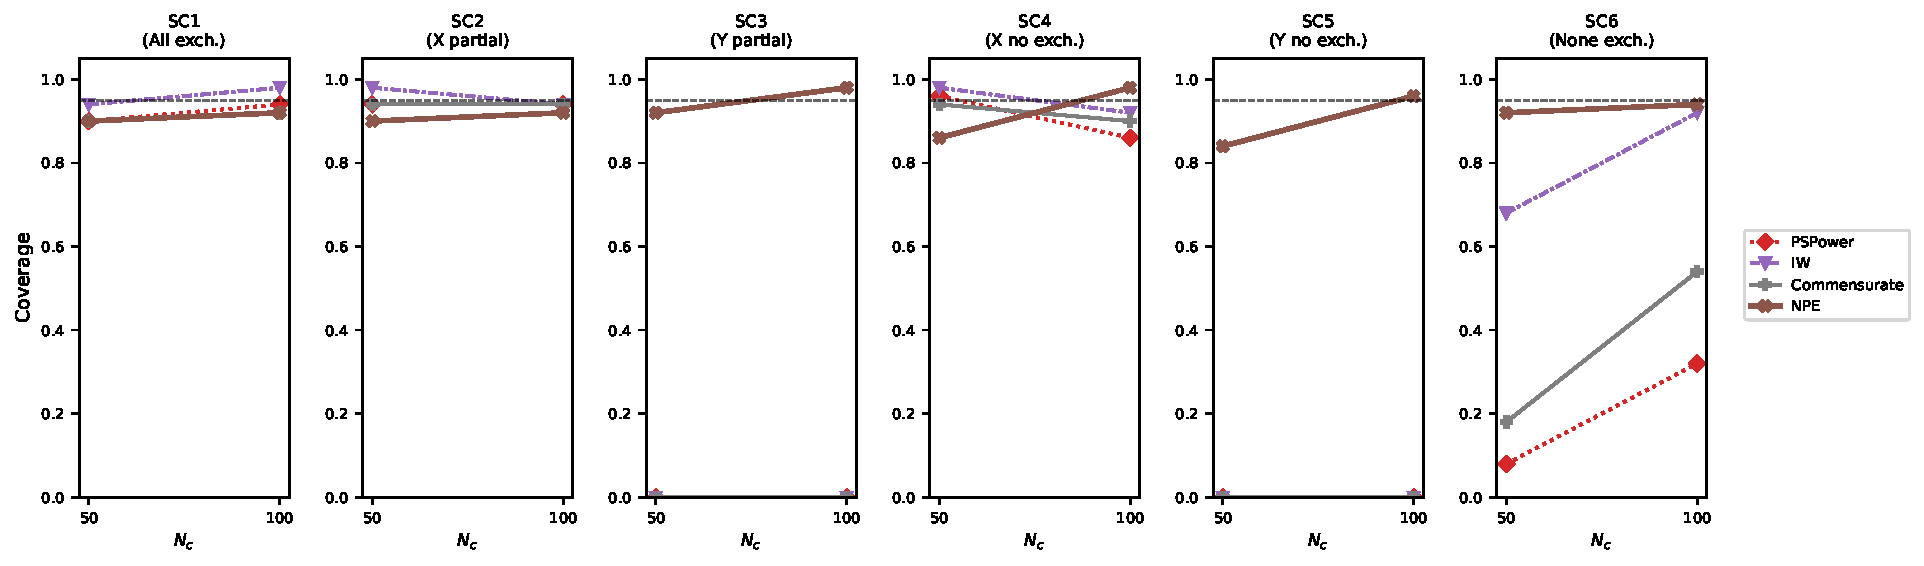
\includegraphics[width=.74\textwidth]{fig_coverage_null.pdf}
    \caption{Coverage across the six simulation scenarios for the null run.}
    \label{fig:sim-coverage-null}
\end{figure}

\begin{figure}[!htbp]
    \centering
    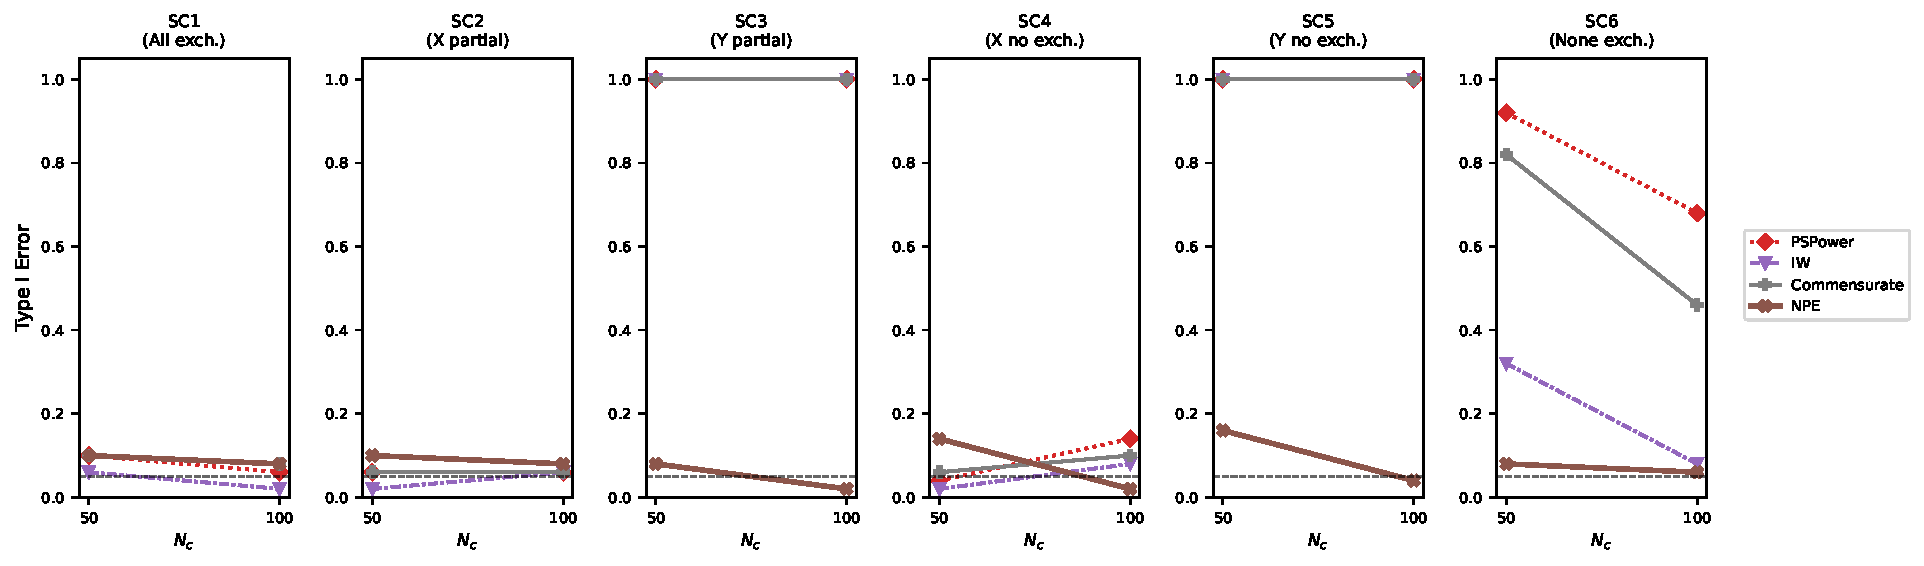
\includegraphics[width=.74\textwidth]{fig_type1_error.pdf}
    \caption{Type I error across the six simulation scenarios for the null run.}
    \label{fig:sim-type1}
\end{figure}

\subsection{Interpretation}

The simulation results do not suggest that NPE is best in every setting.
In SC1 and SC2, and in part of SC4, the classical methods are already stable
and often have smaller bias and RMSE.
The main advantage of NPE appears in the harder settings.
When the outcome model changes across sources, as in SC3 and SC5, or when both
covariate and outcome mismatch are present, as in SC6, the standard borrowing
methods can have large bias, poor coverage, and inflated Type I error.
NPE is much more stable there.

Taken together, these results suggest that NPE is most useful when source
mismatch is difficult to capture with a fixed borrowing rule, especially when the
main problem is outcome drift rather than mild covariate shift.